
\documentclass[calculator,allquestions,datasheet,solutions]{exam_newMarcus2}
%\documentclass[calculator,allquestions,datasheet]{exam_newMarcus2}

% The full list of class options are
% calculator : Allows approved calculator use.
% datasheet : Adds a note that data sheet are attached to the exam.
% handbook : Allows the use of the engineering handbook.
% resit : Adds the resit markings to the paper.
% sample : Adds conspicuous SAMPLE markings to the paper
% solutions : Uses the contents of \solution commands (and \solmarks) to generate a solution file

\usepackage{pdfpages}  
\usepackage{lscape,comment} 
 
\coursecode{EX3029}%%
\coursetitle{Chemical Thermodynamics}
 
\examtime{14.00--17.00}%
\examdate{15}{12}{2016}% 
\examformat{Candidates must attempt \textit{all} questions, each of which carries equal (20) marks.  All thermodynamic symbols have their usual meanings unless otherwise stated.}

\newcommand{\frc}{\displaystyle\frac}
\newcommand{\br}[1]{\!\left( #1 \right)}
\newcommand{\abs}[1]{\left| #1 \right|}
\newcommand{\fracd}[2]{\frac{\mathrm{d} #1}{\mathrm{d} #2}}
\newcommand{\fracp}[2]{\frac{\partial #1}{\partial #2}}
\renewcommand{\d}[1]{\mathrm{d} #1 } 
\newcommand{\Ma}{\mathrm{M\!a}} 



\begin{document}


%%%
%%% Question 01 (Fluid Phase Equilibrium)
%%% LectureNotes_Nguyen (pg 89)
%%%
\begin{question}
The van der Waals equation of state (vdW EOS) is given by,
     \begin{displaymath}
         P = \frc{RT}{V-b} - \frc{a}{V^{2}},
     \end{displaymath} 
     \begin{enumerate}[(a)]
         \item Show that the vdW EOS can be expressed as a cubic polynomial equation in $Z$ (compressibility coefficient),
             \begin{displaymath}
                  Z^{3} -(1+B)Z^{2} +AZ -AB = 0,
             \end{displaymath}
             with $B=bP/(RT)$, $A=aP/(RT)^{2}$ and $R\left(=8.314\times 10^{-5}\frc{\text{bar.m}^{3}}{\text{mol.K}}\right)$ is the molar gas constant~\marks{7}
%==========================
\solution{We can rearrange the vdW EOS,~\solmarks{2/7}
\begin{displaymath}
   P = \frc{RT}{V-b} - \frc{a}{V^{2}} \Longrightarrow \frc{PV}{RT} = \frc{V}{V-b} - \frc{a}{RTV} = \frc{1}{1-\frc{b}{V}} - \frc{a}{RTV}
\end{displaymath}
Eliminating $V$ as $V=ZRT/P$,~\solmarks{1/7}
\begin{displaymath}
   Z = \left(1-\frc{bP}{ZRT}\right)^{-1} - \frc{aP}{Z\left(RT\right)^{2}} = \frc{ZRT}{ZRT-bP}-\frc{aP}{Z\left(RT\right)^{2}}
\end{displaymath}
Manipulating this expression,~\solmarks{3/7}
\begin{eqnarray}
   && Z^{2}R^{2}T^{2}\left(ZRT-bP\right) = Z^{2}\left(RT\right)^{3} - aP\left(ZRT-bP\right) \nonumber \\
   && Z^{3} - \frc{bP}{RT}Z^{2} - Z^{2} -\frc{aP}{\left(RT\right)^{2}}Z + ab\frc{P^{2}}{\left(RT\right)^{3}} = 0 \nonumber
\end{eqnarray}
with $B=bP/(RT)$, $A=aP/(RT)^{2}$,~\solmarks{1/7}
\begin{displaymath}
Z^{3} -(1+B)Z^{2} +AZ -AB = 0 
\end{displaymath}
}
%==========================

\item Calculate the fugacity of gaseous CO$_{2}$ at 310 K and 1.4 MPa using the vdW EOS, with $a=$ 0.3658 Pa.m$^{6}$.mol$^{-2}$, $b=$ 4.286$\times$10$^{-5}$ m$^{3}$.mol$^{-1}$. Given,
\begin{displaymath}
\ln{\left(\frc{f}{P}\right)} = -\ln{\left(1-\frc{b}{V}\right)} - \frc{a}{RTV} - \ln{Z} +\left(Z-1\right).
\end{displaymath}
Use the largest real root of the cubic polynomial equation in $Z$ to represent the gaseous phase.~\marks{13}

%====================
\solution{Solving the cubic polynomial in $Z$, with $B=bP/(RT)$ and $A=aP/(RT)^{2}$,~\solmarks{5/13}
\begin{eqnarray}
Z^{3} -(1+B)Z^{2} +AZ -AB = 0 & \Longrightarrow& A = 7.7095\times 10^{-2}\; ;\; B = 2.3281\times 10^{-2} \nonumber \\ 
 &\Longrightarrow& Z = 0.9436 \nonumber
\end{eqnarray}
Now for the fugacity equation, either
\begin{eqnarray}
&& \ln{\left(\frc{f}{P}\right)} = -\ln{\left(1-\frc{b}{V}\right)} - \frc{a}{RTV} - \ln{Z} +\left(Z-1\right) \nonumber \\
&& \text{or} \nonumber \\
&&  \ln{\left(\frc{f}{P}\right)} = -\ln{\left(1-\frc{B}{Z}\right)} - \frc{A}{Z} - \ln{Z} +\left(Z-1\right) \nonumber
\end{eqnarray}
leads to $f =\; 1.32\times 10^{6}$ Pa.~\solmarks{8/13}

}
%====================
%
\end{enumerate}
%
\end{question}

\clearpage


%%%
%%% Question 02
%%%
\begin{question}
In a saturated liquid mixture of benzene and toluene containing 45 mol$\%$ of benzene, determine:
\begin{enumerate}[(a)]
%
   \item Temperature and composition of the first bubble at 200 kPa.~\marks{10}
%======================
         \solution{ The molar constraint of vapour composition is~\solmarks{1/10}
\begin{displaymath}
   \sum\limits_{i=1}^{2}y_{i} = y_{1} + y_{2} = 1,
\end{displaymath}
and replacing the Raoult law, $y_{i}=\frac{x_{i}P_{i}^{\text{sat}}}{P}$, in the constraint relation,~\solmarks{1/10}
\begin{eqnarray}
   P &=& x_{1}P_{1}^{\text{sat}} + x_{2}P_{2}^{\text{sat}} \nonumber \\
     &=& x_{1}\exp{\left(A_{1}-\frc{B_{1}}{T+C_{1}}\right)} + x_{2}\exp{\left(A_{2}-\frc{B_{2}}{T+C_{2}}\right)}  \nonumber
\end{eqnarray}
Solving this non-linear equation we obtain the bubble temperature of the benzene-toluene mixture as $T=391.79$ K.~\solmarks{3/10} In order to calculate the compositions, we should use the Raoult's relation with P$_{1}^{\text{sat}} = 289.01$ kPa~\solmarks{1/10},~\solmarks{4/10}
\begin{displaymath}
     y_{1} = \frc{x_{1}P_{1}^{\text{sat}}}{P} = 0.6503 \Longrightarrow y_{2} = 0.3497
\end{displaymath}
}
%
   \item Pressure and composition of the first bubble at 400 K.~\marks{10}
%======================
         \solution{ The molar constraint of vapour composition is~\solmarks{1/10}
\begin{displaymath}
   \sum\limits_{i=1}^{2}y_{i} = y_{1} + y_{2} = 1,
\end{displaymath}
and replacing the Raoult law, $y_{i}=\frac{x_{i}P_{i}^{\text{sat}}}{P}$, in the constraint relation,~\solmarks{1/10}
\begin{eqnarray}
   P &=& x_{1}P_{1}^{\text{sat}} + x_{2}P_{2}^{\text{sat}} \nonumber \\
     &=& x_{1}\exp{\left(A_{1}-\frc{B_{1}}{T+C_{1}}\right)} + x_{2}\exp{\left(A_{2}-\frc{B_{2}}{T+C_{2}}\right)}  \nonumber
\end{eqnarray}
Solving this equation for $T = 400$ K results in $P=245.28$ kPa.~\solmarks{3/10} In order to calculate the compositions, we should use the Raoult's relation with P$_{1}^{\text{sat}} = 352.16$ kPa~\solmarks{1/10},~\solmarks{4/10}
\begin{displaymath}
     y_{1} = \frc{x_{1}P_{1}^{\text{sat}}}{P} = 0.6461 \Longrightarrow y_{2} = 0.3539
\end{displaymath}

 }

%
\end{enumerate}

For this problem, benzene and toluene mixtures may be considered as ideal and you should use,
\begin{displaymath}
   \ln P_{i}^{\text{sat}} = A_{i} - \frc{B_{i}}{T + C}
\end{displaymath} 
with [P] = kPa, [T] = K, [B] = K and [C] = K.
    \begin{center}
       \begin{tabular}{l | c c c}   
           {\bf Species}  &   {\bf A } &  {\bf B } &  {\bf C } \\
           \hline
             Benzene (1)  &  14.1603   &  2948.78  & -44.5633  \\
             Toluene (2)  &  14.2515   &  3242.38  & -47.1806   
       \end{tabular}
    \end{center}
%
\end{question}

\clearpage



%%%
%%% Question 05
%%%
\begin{question}
%
  Consider the following chemical reaction representing the chemical equilibrium between dinitrogen tetroxide, N$_{2}$O$_{4}$(g), and nitrogen dioxide, NO$_{2}$(g) at 25$^{\circ}$C and 1 atm, 
       \begin{displaymath}
            N_{2}O_{4}\text{(g)} \Leftrightarrow 2 NO_{2}\text{(g)}.
       \end{displaymath}
Determine:
%
  \begin{enumerate}[(a)]
%
      \item Equilibrium constant of this reaction.~\marks{8}
%======================
         \solution{ The reaction $N_{2}O_{4}\text{(g)} \Leftrightarrow 2 NO_{2}\text{(g)}$ may be obtained by combining reactions (1) and (2), i.e.,~\solmarks{2/8}
                \begin{displaymath}
                     \text{(1) + 2(2)} \Longrightarrow N_{2}O_{4}\text{(g)} \Leftrightarrow 2 NO_{2}\text{(g)}
                \end{displaymath}
            Thus, the standard free Gibbs energy change of the mixture at 25$^{\circ}$C can be obtained from the~\solmarks{3/8}
              \begin{displaymath}
                  \Delta G^{\circ}_{298} =  \Delta G^{\circ}_{1} + 2 \Delta G^{\circ}_{2} = 4478.86 \text{ J.mol}^{-1}
              \end{displaymath}
           The equilibrium constant at 25$^{\circ}$C is given by~\solmarks{3/8} 
          \begin{displaymath}
              K_{\text{eq},298} = \exp{\left[-\frc{\Delta G^{\circ}_{298}}{R T}\right]} = 0.1641
          \end{displaymath}
}
% 
         \item Equilibrium composition of N$_{2}$O$_{4}$(g).~\marks{12}
%======================
         \solution{ The equilibrium constant can also be obtained as a function of the species' activities,~\solmarks{2/12}
             \begin{displaymath} 
                 K = \frc{a^{2}_{NO_{2}}}{a_{N_{2}O_{4}}} = \frc{\left(\frc{\hat{f}_{NO_{2}}}{f^{\circ}_{NO_{2}}}\right)^{2}}{\left(\frc{\hat{f}_{N_{2}O_{4}}}{f^{\circ}_{N_{2}O_{4}}}\right)}
             \end{displaymath}
             Assuming ideal gas behaviour, $\hat{f}_{i}=P_{i}$, $f^{\circ}_{i}=P^{\circ}_{NO_{2}}=P^{\circ}_{N_{2}O_{4}} =$ 1 atm,~\solmarks{2/12}
             \begin{displaymath} 
                 K = \frc{a^{2}_{NO_{2}}}{a_{N_{2}O_{4}}} = \frc{\left(\frc{\hat{f}_{NO_{2}}}{f^{\circ}_{NO_{2}}}\right)^{2}}{\left(\frc{\hat{f}_{N_{2}O_{4}}}{f^{\circ}_{N_{2}O_{4}}}\right)} = \frc{\left(\frc{P_{NO_{2}}}{P^{\circ}_{NO_{2}}}\right)^{2}}{\left(\frc{P_{N_{2}O_{4}}}{P^{\circ}_{N_{2}O_{4}}}\right)} = \frc{\left(\frc{P.y_{NO_{2}}}{1\text{ atm}}\right)^{2}}{\left(\frc{P.y_{N_{2}O_{4}}}{1 \text{ atm}}\right)}  
             \end{displaymath}
             As $P=$ 1 atm,~\solmarks{1/12}
             \begin{displaymath} 
                 K = \frc{\left(\frc{P.y_{NO_{2}}}{1\text{ atm}}\right)^{2}}{\left(\frc{P.y_{N_{2}O_{4}}}{1 \text{ atm}}\right)}  = \frc{y^{2}_{NO_{2}}}{y_{N_{2}O_{4}}} 
             \end{displaymath}
             During the reaction,~\solmarks{1/12}
              \begin{center}
                   \begin{tabular}{c | c c c}
                                   & N$_{2}$O$_{4}$  & NO$_{2}$  & Total \\
                         Initial   &  1            &  0        &  1    \\
                         Final     &  1 - $\xi$    &  2$\xi$   & 1 + $\xi$       
                   \end{tabular}
              \end{center}
              The mole fractions of N$_{2}$O$_{4}$ and NO$_{2}$ can be expressed as~\solmarks{2/12}
              \begin{displaymath}
                  y_{N_{2}O_{4}} = \frc{1-\xi}{1+\xi} \hspace{2cm}\text{ and }\hspace{2cm} y_{NO_{2}}= \frc{2\xi}{1+\xi}
              \end{displaymath}
              and be replaced in the previous equation with $K_{\text{eq},298}= 0.1641$ (from (a))~\solmarks{2/12}
              \begin{displaymath}
                 K =  \frc{y^{2}_{NO_{2}}}{y_{N_{2}O_{4}}} = \frc{\left(\frc{2\xi}{1+\xi}\right)^{2}}{\frc{1-\xi}{1+\xi}} = 0.1641 \Longrightarrow \xi = 0.1985
             \end{displaymath}
            The equilibrium composition is $y_{N_{2}O_{4}}=0.6688$ and $y_{NO_{2}}=0.3312$.~\solmarks{2/12}
}
%
  \end{enumerate}
%

        For this problem, you should consider the following reaction data:   
       \begin{center}
          \begin{tabular}{c l l l}
             (1) &$N_{2}O_{4}\text{(g)}\Leftrightarrow N_{2}\text{(g)} + 2O_{2}\text{(g)}$; & $\left(\Delta G^{\circ}_{f,298}\right)_{N_{2}O_{4}}$ & =  -97.9908 kJ.mol$^{-1}$  \\
% & $\Delta G^{\circ}_{\text{mix},1} = -\left(\Delta G^{\circ}_{f,298}\right)_{N_{2}O_{4}}$ & =  23.41 kcal.mol$^{-1}$  \\
             (2) & $0.5N_{2}\text{(g)}+O_{2}\text{(g)}\Leftrightarrow NO_{2}\text{(g)}$; & $\left(\Delta G^{\circ}_{f,298}\right)_{NO_{2}}$ & = 51.2348 kJ.mol$^{-1}$ 
%$\Delta G^{\circ}_{\text{mix},2} = \left(\Delta G^{\circ}_{f,298}\right)_{NO_{2}}$ & = 12.24 kcal.mol$^{-1}$ 
          \end{tabular}
       \end{center}
          where $G^{\circ}_{f,298}$ is the standard molar free Gibbs energy of formation. Also, the equilibrium constant at 25$^{\circ}$C is given by
          \begin{displaymath}
              K_{\text{eq},298} = \exp{\left[-\frc{\Delta G^{\circ}_{298}}{R T}\right]}
          \end{displaymath}
          where $R\left(=8.314\frc{\text{J}}{\text{mol.K}}\right)$ is the molar gas constant and $\Delta G^{\circ}_{298}$ is the standard free Gibbs energy change of the mixture. Assume ideal gas behaviour.
%
\end{question}

\clearpage


%%%
%%% Question 06
%%%
\begin{question}
%
   \begin{enumerate}[(a)]
%
     \item Two litres of an anti-freezing solution is needed for a cooling process. The solution is prepared by mixing 30$\%$-mol of methanol in water. What are the volumes of pure methanol and water at 25$^{\circ}$C necessary to prepare solution? Partial molar volumes $\left(\overline{V}\right)$ for methanol and water in a 30$\%$-mol of methanol solution and their pure species molar volumes $\left(V\right)$, both at 25$^{\circ}$C are:~\marks{8}
       \begin{center}
          \begin{tabular}{ l l l }
                             & $\overline{V}_{i} \left(\text{cm}^{3}.\text{mol}^{-1}\right)$ & $V_{i} \left(\text{cm}^{3}.\text{mol}^{-1}\right)$ \\
               Methanol (1)  & 38.6320                                                     & 40.7270  \\
               Water (2)     & 17.7650                                                     & 18.0680 
          \end{tabular}
       \end{center}
%======================
         \solution{ The molar volume of the 30$\%$-mol of methanol solution is given by,~\solmarks{2/8}
                  \begin{eqnarray}
                     V &=& \frc{V^{T}}{n_{T}} = \frc{\sum\limits_{i=1}^{2}n_{i}\overline{V}_{i}}{n_{T}} = \sum\limits_{i=1}^{2}x_{i}\overline{V}_{i} = x_{1}\overline{V}_{1} + x_{2}\overline{V}_{2} \nonumber \\
                       &=& (0.3)(38.6320) + (0.7)(17.7650) = 24.0251 \text{ cm}^{3}.\text{mol}^{-1} \nonumber
                  \end{eqnarray}
             The total number of moles are:~\solmarks{2/8}
                  \begin{displaymath}
                      n_{T} = \frc{V^{T}}{V} = \frc{2000}{24.0251} = 83.2463 \text{ mol}
                  \end{displaymath}
             The volume of pure methanol and water for the solution are:~\solmarks{4/8}
                  \begin{eqnarray}
                       && V^{\text{pure}}_{1}= x_{1}n_{T}V_{1} = 1017.11\text{ cm}^{3}\nonumber \\
                       && V^{\text{pure}}_{2}= x_{2}n_{T}V_{2} = 1052.87\text{ cm}^{3}\nonumber 
                  \end{eqnarray}
}
%
      \item In generating expressions from $G^{E}/RT$ from VLE data, a convenient approach is to plot values of $G^{E}/\left(x_{1}x_{2}RT\right)$ {\it vs} $x_{1}$ and fitting results with an appropriate function. Consider if such data were fit by the expression,
   \begin{displaymath}
       \frc{G^{E}}{x_{1}x_{2} R T} = A + B x_{1}^{2}.
   \end{displaymath}
         From the expression $G^{E}/\left(x_{1}x_{2}RT\right)$, provide equations for the activity coefficient, $\ln{\gamma_{i}}$, as a function of $A$, $B$, $x_{1}$ and $x_{2}$, given~\marks{12}
       \begin{displaymath}
               \ln{\gamma_{i}} = \frc{\overline{G}_{i}^{E}}{RT}.
       \end{displaymath} 
%======================
         \solution{ For a binary mixture:~\solmarks{2/12}
             \begin{displaymath}
                  \overline{M}_{1} = M + x_{2}\frc{\d M}{\d x_{1}} \hspace{2cm} \text{ and } \hspace{2cm} \overline{M}_{2} = M - x_{1}\frc{\d M}{\d x_{1}}
             \end{displaymath}
             thus~\solmarks{3/12}
             \begin{displaymath}
                 \ln{\gamma_{1}} = \frc{\overline{G}^{E}_{1}}{RT} = \frc{G^{E}}{RT} + x_{2}\frc{\d G^{E}/RT}{\d x_{1}} \;\text{ and }\; \ln{\gamma_{2}} = \frc{\overline{G}^{E}_{2}}{RT} = \frc{G^{E}}{RT} - x_{1}\frc{\d G^{E}/RT}{\d x_{2}}
             \end{displaymath}
             with~\solmarks{5/12}
             \begin{displaymath}
                 \frc{\d G^{E}/RT}{\d x_{1}} = \left(1-2x_{1}\right)A + \left(3-4x_{1}\right)Bx_{1}^{2}
             \end{displaymath}
             The activity coefficient is then given by,~\solmarks{2/12}
             \begin{eqnarray}
                  && \ln{\gamma_{1}} = x_{1}\left(1-x_{1}\right)\left(A+Bx_{1}^{2}\right) + \left(1-x_{1}\right)\left[\left(1-2x_{1}\right)A + \left(3-4x_{1}\right)Bx_{1}\right] \nonumber \\
                  && \ln{\gamma_{2}} = x_{1}\left(1-x_{1}\right)\left(A+Bx_{1}^{2}\right) + x_{1}\left[\left(1-2x_{1}\right)A + \left(3-4x_{1}\right)Bx_{1}\right] \nonumber 
             \end{eqnarray}
                
}
%
   \end{enumerate}
%
\end{question}

\clearpage

%%%
%%% QUESTION 5
%%%
\begin{question}
\begin{enumerate}[(i)]
% SM&VN 10.13
\item A concentrated binary solution containing mainly species $2$ $\left(\text{though } x_{2}\not= 1\right)$ is in equilibrium with a vapour phase containing both species $1$ and $2$. Pressure and temperature of this two-phase system are 1 bar and 298.15 K. Given $\mathcal{H}_{1}$ = 200 bar (Henry constant) and P$_{2}^{\text{sat}}$ = 0.10 bar, calculate $x_{1}$ and $y_{1}$.~\marks{10}
%
\solution{Assuming that at 1 bar the vapour phase behaves as an ideal gas. The vapour phases fugacities are then equal to the partial pressures. Assume the Lewis/Randall rule applies to concentrated species $2$ and that Henry's law applies to dilute species $1$, therefore,
\begin{displaymath}
y_{1}P=\mathcal{H}_{1}x_{1};\;\;\text{ and }\;\; y_{2}P= x_{2}P_{2}^{\text{sat}}
\end{displaymath}
with $x_{1}+x_{2}=1$. Thus $P = y_{1}P + y_{2}P$ becomes,~\solmarks{5/10}
\begin{displaymath}
P = \mathcal{H}_{1}x_{1}+\left(1-x_{1}\right)P_{2}^{\text{sat}} \;\;\Longrightarrow {\bf x_{1} = 4.502\times 10^{-3}}
\end{displaymath}
and ${\bf y_{1}=\frc{\mathcal{H}_{1}x_{1}}{P}=0.9}$.~\solmarks{5/10}
}
%
% SM&VN 10.19
\item Chemical species $A$ and $B$ are in vapour-liquid equilibrium at 298.15 K. The following conditions are applied to this system:\begin{center}
\begin{tabular}{l l l}
             &  $\mathbf{P_{i}^{\text{sat}}}$ (bar)  &  $\mathbf{\ln{\gamma_{i}}}$\\
    \hline
    {\bf A}  &    1.24                           & 1.8 $x_{B}^{2}$   \\
    {\bf B}  &    0.89                           & 1.8 $x_{A}^{2}$
\end{tabular} 
\end{center}
Assuming that $y_{i}P = x_{i}\gamma_{i}P_{i}^{\text{sat}}$ (where $\gamma_{i}$ is the activity coefficient of species $i$) is valid, calculate the pressure $P$ and the vapour mole fraction $y_{A}$ for a liquid mole fraction of $x_{A}=0.65$.~\marks{10}
%
\solution{With $x_{A}$ =0.65 and $x_{B}$=0.35, we can calculate the activity coefficients, $\gamma_{A}$ and $\gamma_{B}$, and apply in~\solmarks{5/10}
     \begin{displaymath}
         P = x_{A}\gamma_{A} P_{A}^{\text{sat}} + x_{B}\gamma_{B} P_{B}^{\text{sat}} =  1.671 \text{ bar}.
     \end{displaymath}
The vapour mole fraction is obtained from~\solmarks{5/10}
     \begin{displaymath} 
          y_{A} = \frc{x_{A}\gamma_{A}P_{A}^{\text{sat}}}{P} = 0.6013
     \end{displaymath}
} 

\end{enumerate}

\end{question}


\vfill
\paperend



\vfill 



%\begin{comment}
{
  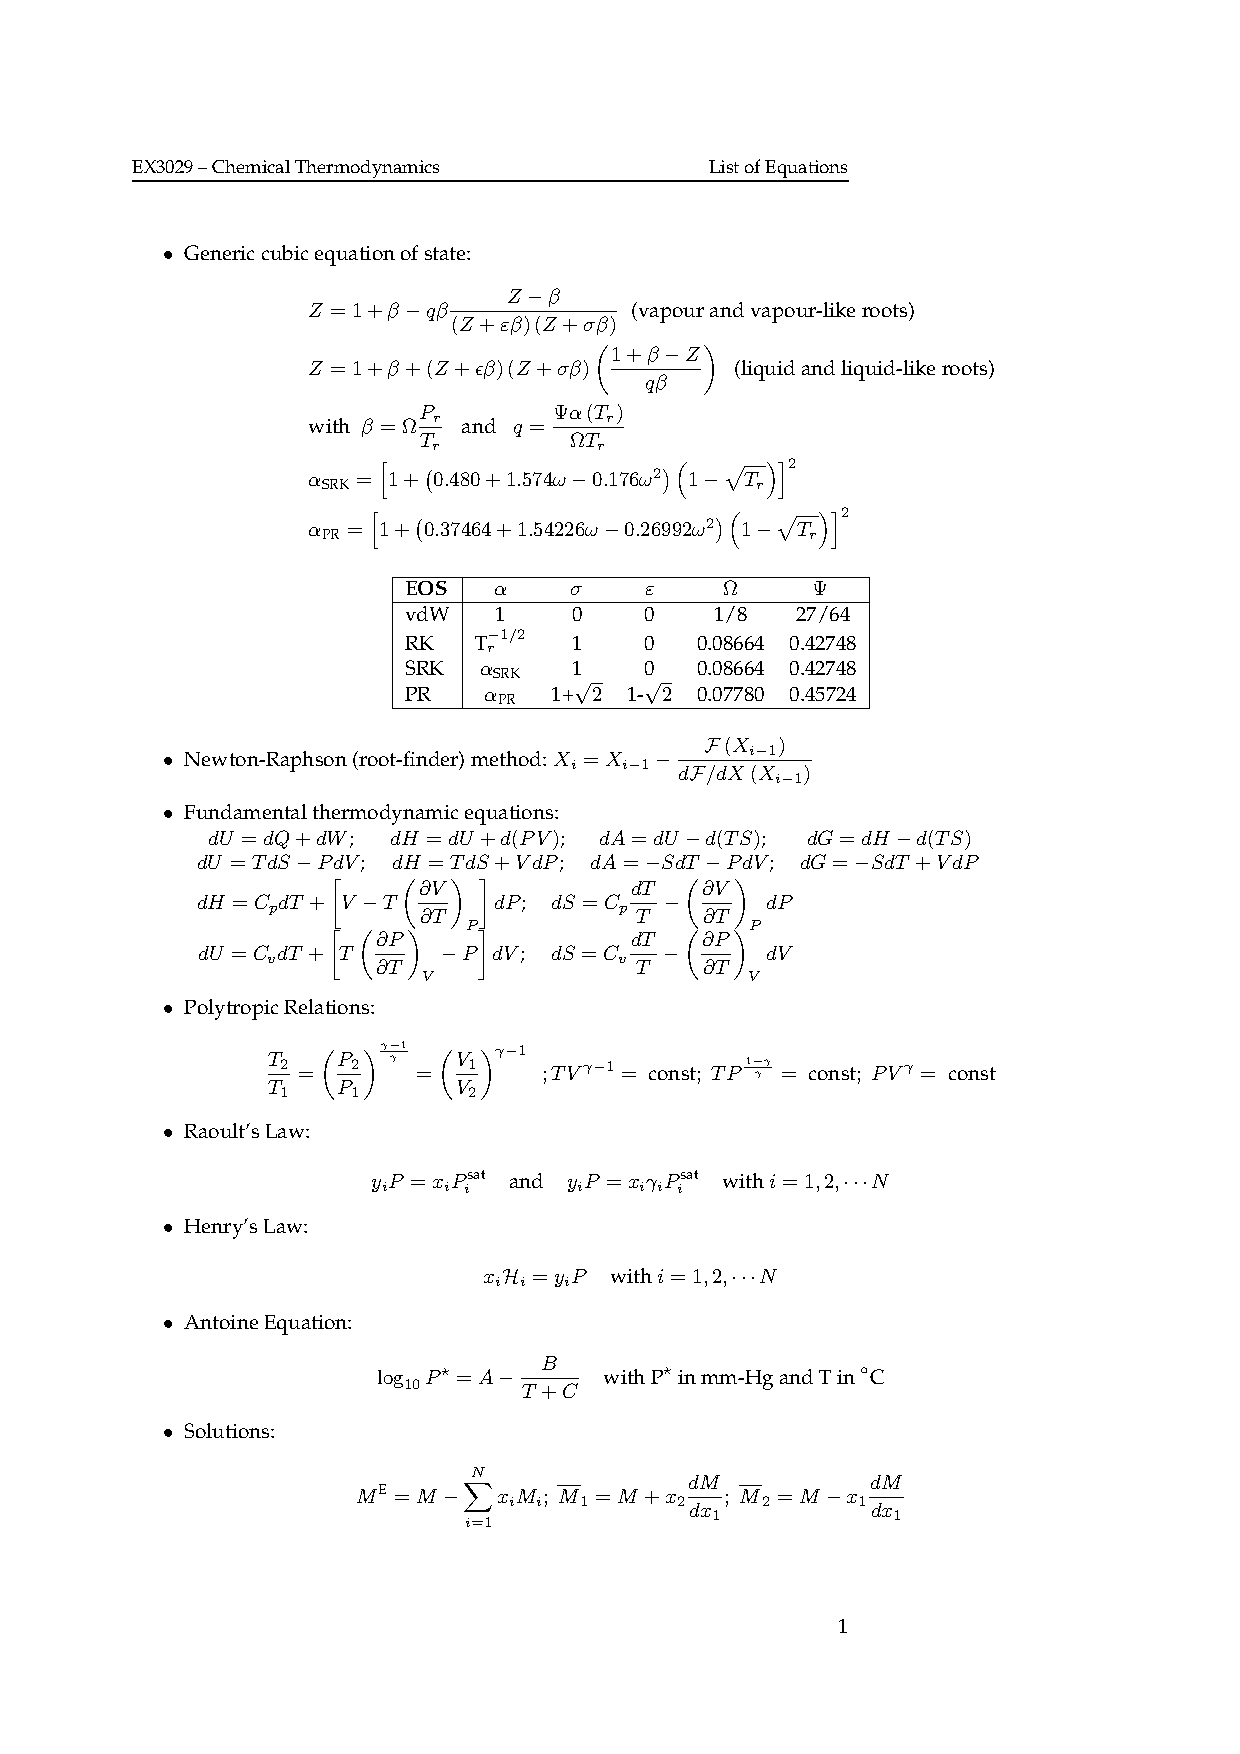
\includepdf[pages=-,fitpaper]{./Pics/EquationsList}
  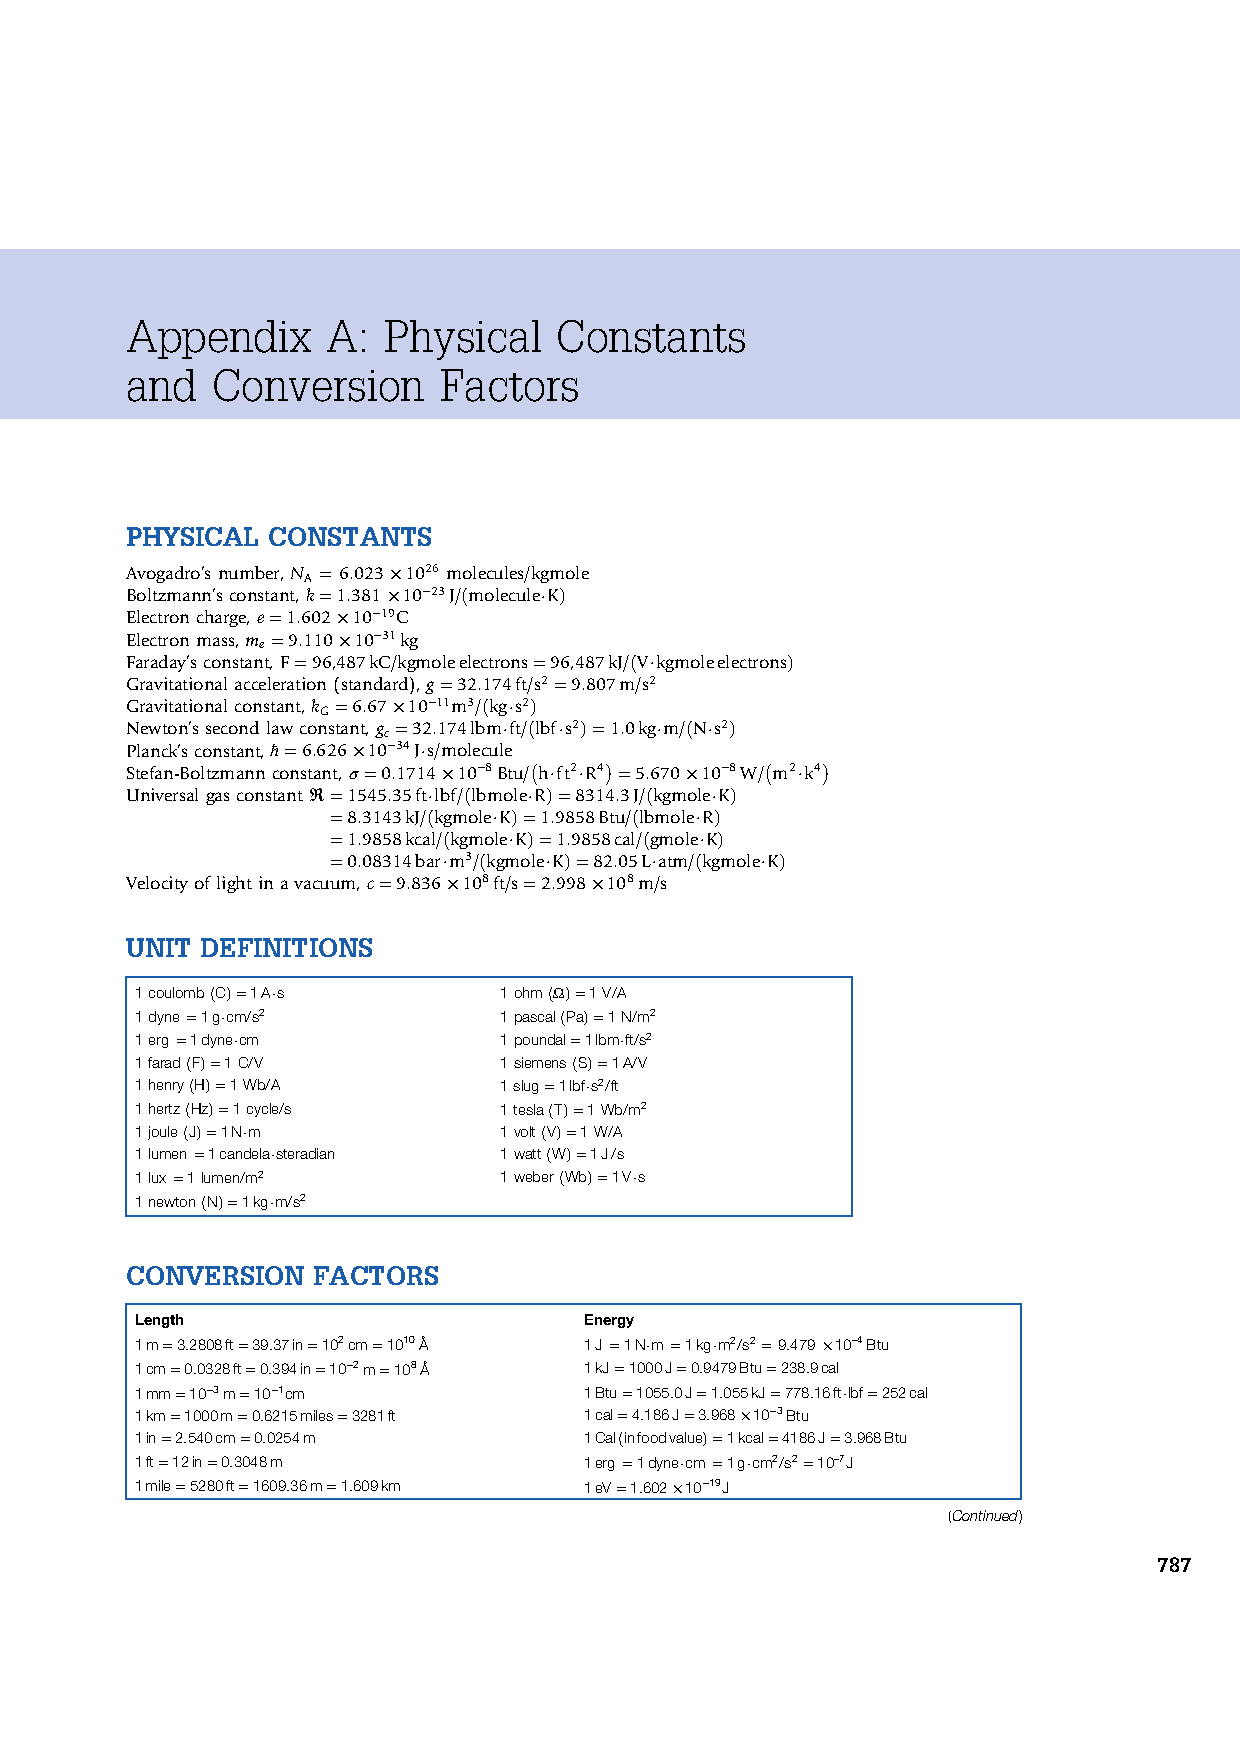
\includepdf[pages=-,fitpaper]{./Pics/ChemEng_UnitConv}
}
%\end{comment}



\end{document}
